\documentclass{report}
\usepackage{import}

\import{.}{preamble.tex}

%\author{Artur Salawa}
%\date{\today{}}
\begin{document}

\begin{titlepage}
	\begin{center}
        
		\large
		\textbf{Jagiellonian University}\\
		Department of Theoretical Computer Science\\

		\vspace{1.5cm}

		\Large
		\textbf{Artur Salawa}

		\vspace*{2cm}

		\textbf{\LARGE Implementation of exponential algorithms for the independent set  problem}
		
		\vspace{0.5cm}
		\large
		
		\vfill
		\Large
		Bachelor's Thesis

		\vfill
		\Large
		Supervisor: dr hab. in\.z. Krzysztof Turowski
		
		\vspace{0.8cm}
		
		August 2023
		
\end{center}
\end{titlepage}
\pagebreak

%\begin{abstract}
%Maximum Independent Set problem also known as \textbf{MIS} has been studied for almost half a century. The first article on Maximum independent set was published in 1977 by Tarjan and Trojanowski \cite{tarjan1977finding} and reached running time of $O^*(2^{n/3}) = O^*(1.2599^n)$. However, earlier than that one can find publications on the counting the Maximal independent sets and similar problems that had solutions faster than $O(2^n)$. Using ideas from these algorithms it is quite easy to derive an algorithm for MIS but it seems like the MIS was not a subject of study yet. Currently the fastest solution was published in 2017 by Mingyu Xiao and Hiroshi Nagamochi running in $O^*(2^{0.2626n})=O^*(1.1996^n)$ \cite{xiao2017exact}.

%In chapter 1 we start with basic definitions. In chapter 2 we introduce naive approach and other simple algorithms. Chapter 3 discusses more advanced algorithms. In the last chapter 4 we present practical running times of the implemented algorithms in an open source Koala NetworKit library.

%\end{abstract}

\tableofcontents

\pagebreak

\chapter{Introduction}
\section{Definitions}

We first give some basic definitions in graph theory sourced from~\cite{bollobás1998modern}.

\begin{defn}[graph]
    A \emph{graph} $G$ is an ordered pair of disjoint sets $(V, E)$ such that $E$ is a subset of the set $V \choose 2$ of unordered pairs of $V$. 
\end{defn}

We only consider finite graphs, that is, $V$ and $E$ are always finite. The set $V$ is the set of \emph{vertices} and $E$ is the set of \emph{edges}. If $G$ is a graph, then $V = V(G)$ is the \emph{vertex set} of $G$, and $E = E(G)$ is the \emph{edge set} of $G$. If $v$ is a vertex of $G$ we will sometimes write $v \in G$ instead of $v \in V(G)$. 

We denote $n_G = |V(G)|$ and $m_G = |E(G)|$ for a graph $G = (V, E)$. We will drop the subscripts for brevity when $G$ is clear from the context.

An edge $\{ x, y \}$ is said to \emph{join} the vertices $x$ and $y$ and is denoted $xy$. Thus, $xy$ and $yx$ mean exactly the same edge, the vertices $x$ and $y$ are the \emph{endvertices} of this edge. If $xy \in E(G)$, then $x$ and $y$ are \emph{adjacent}, \emph{neighboring} or \emph{connected}, and the  vertices $x$ and $y$ are \emph{incident} with the edge $xy$. Two edges are \emph{adjacent} if the have exactly one common endvertex.

The set of vertices adjacent to a vertex $v \in G$.

\begin{defn}[subgraph]
    We say that $G' = (V', E')$ is a \emph{subgraph} of $G = (V, E)$ if $V' \subseteq V$ and $E' \subseteq E$. In this case we write $G' \subseteq G$. If $G'$ contains all edges of $G$ that join two vertices in $V'$ then $G'$ is said to be a subgraph \emph{induced} or \emph{spanned} by $B'$ and is denoted $G[V']$. 
\end{defn}

For a subgraph $G' = G[H]$ spanned by a vertex subset $H \subseteq V(G)$, we write $n_H = |H|$ and $m_H = |E(G')|$.

If $W \subseteq V(G)$, then $G - W = G[V \setminus W]$ is the subgraph of $G$ obtained by deleting the vertices of $W$ and all edges incident with them. Similarly, if $E' \subseteq E(G)$, then $G - E' = (V(G), E(G) \setminus E')$. If $W = \{ w \}$ and $E' = \{ xy \}$ for some vertex $w \in V(G)$ and edge $xy \in E(G)$, then the notation is simplified to $G - w$ and $G - xy$. Similarly, if $x$ and $y$ are nonadjacent vertices of $G$, then $G + xy = (V(G), E(G) \cup \{ xy \})$.

\begin{defn}[path]
    A \emph{path} is a graph $P$ of the form

    \begin{align*}
        V(P) &= \{x_0, x_1, \dots, x_l\} \\
        E(P) &= \{x_0x_1, x_1x_2, \dots, x_{l-1}x_l\}
    \end{align*}
\end{defn}

This path $P$ is usually denoted by $x_0x_1\dots x_l$. The vertices $x_0$ and $x_l$ are the \emph{ends} of $P$ and the value $l = |E(P)|$ is the \emph{length} of $P$. We say that $P$ goes from $x_0$ to $x_l$.

\begin{defn}[connected graph]
    A graph is \emph{connected} if for every pair $\{x, y\}$ of distinct vertices there is a path from $x$ to $y$.
\end{defn}

A maximal connected subgraph is a \emph{component} of a graph.

\begin{defn}[cycle]
    A \emph{cycle} is a graph $C$ of the form

    \begin{align*}
        V(C) &= \{x_0, x_1, \dots, x_l\} \\
        E(C) &= \{x_0x_1, x_1x_2, \dots, x_{l-1}x_l, x_l x_0\}
    \end{align*}
\end{defn}

This cycle $C$ is denoted by $x_0 x_1\dots x_l x_1$. The value $l + 1 = |E(C)| = |V(C)|$ is the \emph{length} of $C$. 

\begin{defn}[forest, tree]
    A graph without any cycles is a \emph{forest}, or an \emph{acyclic} graph. A \emph{tree} is connected forest.
\end{defn}

\begin{defn}[bipartite graph]
    A graph $G$ is a \emph{bipartite} graph with vertex classes $V_1$ and $V_2$ if $V(G) = V_1 \cup V_2$, $V_1 \cap V_2 = \emptyset$ and every edge joins a vertex of $V_1$ to a vertex of $V_2$.
\end{defn}

An easy observation is that a graph is bipartite if and only if it does not contain an odd-length cycle.

A set of vertices (edges) is \emph{independent} if no two elements of it are adjacent.

\begin{defn}[matching]
    A set of independent edges is called a \emph{matching}. A matching $M$ is \emph{perfect} if every vertex is adjacent to exactly one edge in $M$.
\end{defn}

\begin{defn}[exposed vertices]
    A vertex $v$ is \emph{exposed} for a matching $M$ if it is not adjacent to any edge in $M$. If a vertex is not exposed it is \emph{matched}.
\end{defn}

If a vertex $v$ is matched in a matching $M$, then we call the vertex $u$, such that $uv \in M$, the \emph{mate} or \emph{matched vertex} of $v$ and the edge $\{u, v\}$ the \emph{matched edge} of $v$.

\begin{defn}[alternating path]
    A path $P = x_0x_1\dots x_l$ is alternating for a matching $M$ if for each $i \in \{0, \dots, l - 2\}$, $x_i x_{i+1} \in M$ if and only if $x_{i+1}x_{i+2} \notin M$.
\end{defn}

\begin{defn}[augmenting path]
    An alternating path $x_0x_1\dots x_l$ is \emph{augmenting} if the vertices $x_0$ and $x_l$ are both exposed.
\end{defn}

\begin{defn}[weighted graph]
    A \emph{weighted} graph is a graph $G = (V, E)$ along with a \emph{weight function} $w : E \rightarrow \mathbb{R}$, which assigns a real valued \emph{weight} $w(e)$ to each edge of $G$.
\end{defn}

For a set of edges $S \subseteq E$, we define the \emph{weight} of $S$ to be $w(S) = \sum_{e \in S} w(e)$. 

We denote $N_G = \max_{e \in E} w(e)$ for a graph $G = (V, E)$, which we shorten to $N$ when $G$ is clear from the context. In this work, we consider only graphs with non-negative weights.

The algorithms for the maximum matching problems are usually divided into groups based on the classes of graphs they operate on and the type of matching they find. The graphs can be either bipartite or non-bipartite. When the graphs are unweighted, the algorithms find matchings with maximum number of edges. When they're weighted, a matching with maximum possible weight is sought. In the case of weighted graphs we can also restrict our search to perfect matching, looking for the one with the highest weight. In this work we consider the following variants of the maximum matching problem on general graphs:

\begin{itemize}
    \item \textsc{Maximum Cardinality Matching} (\textsc{MCM}) Find a matching in a graph $G$ with maximum number of edges,
    \item \textsc{Maximum Weight Matching} (\textsc{MWM}) Find a matching in a weighted graph $G$ with maximum weight,
    \item \textsc{Maximum Weight Perfect Matching} (\textsc{MWPM}) Find a perfect matching in a weighted graph $G$ with maximum weight.
\end{itemize}

\begin{theorem}\label{thm:reduction}
The \textsc{MWM} and \textsc{MWPM} problems are reducible to each other.

\begin{proof}
    For an instance $G=(V, E)$ of \textsc{MWM}, define a new graph $G' = (V', E')$ where $V' = V_1 \cup V_2$ consists of two copies of $V$ and the edge set $E'$ contains two copies of $E$ along with zero-weight edges between each corresponding pair of vertices in the two copies of $V$. A maximum weight perfect matching $M'$ on $G'$ can be used to obtain a maximum weight matching $M$ on $G$ by restricting the matching to only edges contained in $V_1$. If a vertex in $V_1$ is matched to its copy in $V_2$, it is unmatched in $M$. It is easy to see that $M$ is a maximum weight matching on $G$ as a matching with higher weight could be used to create a perfect matching on $G'$ with weight higher than $M'$. 
    
    In the other direction, let a graph $G=(V, E)$ with weight function $w$ be an instance of \textsc{MWPM}. Construct a weight function $w'(e) = w(e) + nN$. A maximum weight matching on the graph $G' = G$ with weight function $w'$ must have the maximum possible number of edges as the $nN$ term in the definition $w'$ ensures that any matching with more edges has a higher weight.    
\end{proof}
\end{theorem}

In the case of perfect matchings, sometimes the problem is defined as the \textsc{Minimum Weight Perfect Matching}. It is easy to see that it is equivalent to \textsc{Maximum Weight Perfect Matching}. To reduce an instance of one of the problems consisting of a graph $G = (V, E)$ with a weight function $w$ to an instance of the other, simply create a new weight function $w'(e) = N_G - w(e)$. Similar reduction can be used when the instance of \textsc{Minimum Weight Perfect Matching} contains negative weights, we just need to take into account the difference between the minimum and maximum weights.

\section{Background and motivation}
The main goal of this thesis is to provide a clear and accessible presentation of the most important techniques and ideas behind the algorithms for the single source shortest path problem in planar graphs. By summarizing and comparing different approaches, we aim to give the reader a deeper understanding of how exploiting the structure of planar graphs can lead to significant algorithmic improvements.

Planar graphs possess several theoretical properties that are essential for designing efficient algorithms. For instance, planar graphs are sparse: the number of edges is $O(n)$, as follows from Euler's formula \cite{wiki}. Moreover, by the Planar Separator Theorem \cite{separatorT}, for any planar graph on $n$ vertices, it is possible to find a set of $O(\sqrt{n})$ vertices whose removal separates the graph into smaller, roughly balanced parts. These structural properties will be frequently used throughout this paper.

The single-source shortest path problem is one of the most fundamental and important problems in the family of planar graphs. The solutions presented in this paper may be used to improve the time complexity of various algorithms, such as finding feasible flows and matching in bipartite planar graphs.

The standard algorithm for finding shortest paths in weighted graphs is Dijkstra's algorithm. Its implementation using heap achieves time complexity of $O(n \log n)$ \cite{dijkstraBound}.

In this paper, we will present two algorithms for the single-source shortest path (SSSP) problem in planar graphs: the first is proposed by Greg Frederickson in 1986 \cite{frederickson}, achieving time complexity of $O(n \sqrt{\log n}) $, and the second is a simplified version of algorithm proposed by Monika Henzinger \cite{henzinger}, which achieves time complexity of $O(n \log \log n)$. Both of these algorithms are based on Dijkstra algorithm, but they additionally exploit properties of planar graphs to significantly reduce asymptotic running time. Currently, the best-known algorithm and also the one that achieves theoretical lower bound for finding the shortest path to every node in planar graphs is the SSSP algorithm from \cite{henzinger}, which runs in $O(n)$ time.

We will now briefly describe the Dijkstra algorithm to provide necessary intuition for understanding the proofs presented later in this paper. The main idea behind Dijkstra's algorithm serves as a foundation for more complex algorithms for planar graphs.

Dijkstra's algorithm computes the shortest path from a single source vertex $s$ to all other vertices in a weighted graph with non-negative edge weights. The algorithm maintains a set of vertices whose shortest distance from the source has already been determined, and for every other vertex $v$, it keeps track of the current best known distance $p(v)$ from $s$ to $v$.
Initially all vertices are open, $p(s) = 0$ and $p(v) = \infty$ for all $v \neq s$. Algorithm in each iteration closes the open vertex $v$ with the smallest $p(v)$ and relaxes all edges outgoing from $v$. That is, for every neighbor $w$ of $v$, the algorithm updates $p(w)$ if a shorter path from $s$ to $w$ via $v$ is found.

The distances $p(v)$ can be maintained in a heap, which allows for $O(\log n)$ time per update. Since there are $O(n)$ heap updates, and each edge is relaxed at most once, the total running time is $O(n \log n)$ \cite{dijkstraBound}.

One approach to reducing the asymptotic running time of shortest path algorithms is to minimize the maximum number of nodes present in the heap at any given time. This means that a preprocessing phase is necessary to identify this subset of vertices a heap will be used on. How can we exploit properties of planar graphs to achieve this goal? The key idea shared by both of the algorithms presented in this paper is to partition the graph into appropriate sized regions during the prepossessing phase. In Chapter 2, we will describe the specific properties that such a division must have in order to take advantage of the structure of planar graphs, as well as how to construct this partition efficiently. Once the partitioning is completed, the algorithm must carefully coordinate heap updates between the regions to avoid increasing the total number of heap operations. In Chapters 3 and 4, we will explain the approaches taken by each of the two algorithms in detail.


\section{General method for estimating an upper-bound}

To determine complexities of algorithms we will be using these two asymptotic notions, deriving from the Landau big-O notation:
\begin{defn}[Big $O$]
$\boldsymbol{O(g(n))}$ is defined as: \\
$O(g(n)) = \{ f (n) \colon$ there exist positive constants $c$ and $n_0$ such that
$0 \leq f (n) \leq cg(n)$ for all $n \geq n_0\}$
\end{defn}

\begin{defn}[Big $\Theta$]
$\boldsymbol{\Theta(g(n))}$ is defined as: \\
$O(g(n)) = \{ f (n) \colon$ there exist positive constants $c_1, c_2$ and $n_0$ such that
$0 \leq c_1 g(n) \leq f (n) \leq c_2 g(n)$ for all $n \geq n_0\}$
\end{defn}

\begin{defn}[Big $O^*$]
$\boldsymbol{O^*(g(n))}$ is defined as: \\
$O^*(g(n)) = f(n)$ if $f(n) = O(g(n)poly(n))$, where $poly(n)$ is a polynomial.
\end{defn}

Throughout this work, we determine upper bounds on the worst-case running times of our exact exponential algorithms as functions $O^*(\alpha^n)$ and some real constant $\alpha \geq 1$. 

Flow control statements in branching algorithms split entire procedure into so-called reduction rules and branching rules. These rules must have polynomial complexity.

\begin{defn}[reduction rule]
A \emph{reduction rule} simplifies a problem instance or halts the algorithm.
\end{defn}
Reduction rules reduce the size of a current instance. The usually appear before branching rules as they allow for problem simplification without the creation of additional subproblems.

\begin{defn}[branching rule]
A \emph{branching rule} is used to solve a problem instance by recursively solving smaller instances of the problem.
\end{defn}

Let us define a search tree representing an execution of a branching algorithm. We build such trees as follows:
\begin{itemize}
    \item we assign the root node of the search tree to the input of the problem,
    \item we recursively assign a child to a node for each smaller instance reached by applying a branching rule to the current instance state.
\end{itemize}

Let $T(n)$ count the number of leafs of that search tree.
The general approach is to analyze each branching rule separately and then to use the worst-case time over all branching rules as an upper bound on the running time of the algorithm.

Let's take a branching rule $b$ which form instance of size $n$ that creates instances of sizes $n-t_1, n-t_2, \ldots, n-t_n$. We can deduce that $T(n)$ will be bounded by the following:

$$T(n) \leq T(n-t_1) +T(n-t_2) + \ldots +T(n-t_r).$$

With this linear recurrence equation we also associate a \emph{branching vector} $b=(t_1, t_2, \ldots, t_r)$. There are well-known standard techniques to solve linear recurrences, however, in this paper we omit this discussion. 

Important thing to note is that when at least one $t_i$ has $\Theta(n)$ complexity, the complexity of the entire branch is exponential. Linear recurrence associated with branching vector has an unique solution $\alpha$ but it this article we do not focus on techniques facilitating solving linear recurrences. Instead, we will use a function $\tau$ that takes elements of a branching vector as an argument and returns $\alpha$. 

The computational complexity of a branch determined by a branching vector $b=(t_1, t_2, \ldots, t_r)$ is equal to
$O^*(\alpha^n)$ where $\tau(t_1, t_2, \ldots, t_r) = \alpha$. Traditionally we estimate $\alpha$ up to four decimal places. A more detailed description is available in \cite{book}.


\chapter{Simple algorithms}
\section{Naive Algorithm}

The easiest solution to the maximum independent set problem is the naive (otherwise known as the bruteforce) approach. \textsc{MisNaive} algorithm simply checks every possible induced subgraph of the graph $G$. It verifies if this is indeed an independent set and then compares it with the best currently known solution. If the currently analyzed subgraph satisfies these requirements, then the best solution is overwritten.

\begin{algorithm}
\caption{\textsc{MisNaive}}\label{bruteforce}
\begin{algorithmic}[1]
\Require a graph $G=(V,E)$
\Ensure the maximum independent set of $G$
\Procedure{MisNaive}{graph $G$}
    \State $I \gets \emptyset$
    \ForEach {$V' \subseteq V$}
        \If{$G[V']$ has no edge \textbf{and} $|V'| > |R|$}
            \State $I \gets V'$            
        \EndIf
    \EndFor
    \State \Return $I$
\EndProcedure
\end{algorithmic}
\end{algorithm}

\subsection{Correctness}

Algorithms iterate over every single subgraph of a $G$ graph and check if it is independent and bigger than the previously found, so the returned set has to be doubtlessly independent and also maximum.

\subsection{Computational complexity}

There are $2^n$ subsets of the set of size $n$, and checking whether $E'$ does not contain any edge is polynomial in $n$. Therefore, the complexity is $O^*(2^n)$. It is the slowest possible time for a reasonable algorithm, however for small graphs, it could be the fastest approach due to low overhead.
\section{Mis1}

Let us start with a disclaimer that all algorithms presented below, bar the one presented in \Cref{sec:misfolding} are slower than the one published by Tarjan and Trojanowski. Despite that, they are interesting not only from the educational point of view but also as easy-to-implement points of reference for practical measurements -- as it is often the case that in practice simple algorithms may outperform the more convoluted ones with better worst-case guarantees.

Let us start with a definition of neighborhood.

\begin{defn}[neighborhood]
The set of all neighbors of a vertex $v$ of $G = (V, E)$, denoted by $N(v)$, is called the (open) \emph{neighborhood} of $v$.

By $N[v]$ we denote a closed neighborhood that additionally contains a vertex $v$. In mathematical terms, it is $N[v]=N(v) \cup \{v\}$.
\end{defn}
More generally, by $N^d(v)$ we denote the set of nodes at a distance $d$ from $v$. In particular, $N^1(v) = N(v)$.

\begin{lemma}
For any vertex $v\in G$, at least one vertex of $N(v)$ must belong to the maximum independent set of $G$.
\end{lemma}
\begin{proof}
    The proof is very straightforward. Let us assume otherwise that the set $I$ is a maximal independent set of $G$ and in $G$ exists $v$ such that no $N[v]$ belongs to $I$. We can add the vertex $v$ to $I$ and create a larger set than $I$ and also maximum. Hence, a contradiction.
\end{proof}

So, for any vertex $v$ we know that one of the $N[v]$ belongs to the solution. Using that observation, we can create a \textsc{Mis1} algorithm that will hopefully have a better computational complexity than $O^*(2^n)$. 

\begin{algorithm}
\caption{\textsc{Mis1}}\label{mis1}
\begin{algorithmic}[1]
\Require a graph $G=(V,E)$
\Ensure the maximum independent set of $G$
\Procedure{Mis1}{graph $G$}
    \If{$|V| = 0$}
        \State \Return $\varnothing$
    \EndIf
    \State choose arbitrary vertex $v$ of minimum degree in $G$
    \State $S \gets \{ \Call{Mis1}{G \setminus N[y]}\cup \{y\} \colon y \in N[v]\}$
    \State \Return any element of $S$ with the most elements    
\EndProcedure
\end{algorithmic}
\end{algorithm}

\subsection{Correctness}

The algorithm chooses a vertex $v$ and creates $N[v]$ subproblems. Each subproblem is another maximum independent set problem that will have to be solved. We know that some verticle $y$ of $N[v]$ has to be chosen to the independent set, and therefore, one of the subproblems plus the chosen vertex $y$ will give an optimal solution. Eventually, subproblems will be reduced to the size of $0$, and for them in fact, the empty set is the maximal independent set. After recursion finishes, it is going to return some maximal independent set.

Generally, we branch over some cases, reduce the original problem to new subproblems and then analyze them exactly as the original problem. This approach is known as \emph{Branch and Reduce}. 

\subsection{Computational complexity}

For \textsc{Mis1} algorithm, just once, we will do a full analysis of the complexity, including solving a recurrence. 

Let each node of the execution tree represent one call of the recursive function. We will be counting the number of nodes. Let $n$ be a number of vertices of graph $G$ and $T(k)$ be a function counting the maximum size of a branching tree for a graph $G$ consisting of $k$ vertices. We can obtain the following recurrence relation for each node:

$$
T(n) \leq 1 + \sum_{y\in N[v]} T(n - d(y) - 1)
$$

The first $1$ in the equation stands for one call before branching. The sum is over $N[v]$ because we branch over the neighbors of chosen $v$. And finally, $n - d(y) - 1$ is the size of the reduced subproblem. From the above recursive relation, we shall bound running time in $O^*$ terms.

From the choice of $v$ (we are choosing minimum degree vertex) we have $n-d(y)-1 \leq n - d(v) -1$ and from the monotonic property of $T$ we get the following:

\begin{equation*}
\begin{split}
T(n) & \leq 1 + \sum_{y\in N[v]} T(n - d(y) - 1) \\
 & \leq  1 + \sum_{y\in N[v]} T(n - d(v) - 1) \\
 & = 1 + T(n - d(v) - 1) \sum_{y\in N[v]} 1 \\
 & = 1 + T(n - d(v) - 1)(d(v) + 1)
\end{split}
\end{equation*}

Let $s = d(v) + 1$. We obtain the following.

$$
T(n) \leq 1 + s T(n - s)
$$

We can expand $T(n-s)$, and then use $T(0)=1$ and properties of geometric series
\begin{equation*}
\begin{split}
T(n) & \leq 1 + s T(n - s) \\
 & \leq 1 + s + s^2T(n - 2s) \\
 & \leq 1 + s + s^2 + \ldots + s^{n/s - 1} + s^{n/s} T(0) \\
 & = \frac{1-s^{n/s+1}}{1-s} \\
 & = O^*\left(s^{n/s}\right)
\end{split}
\end{equation*}

Since $s^{n/s} = (s^{1/s})^n$, it is enough to find the maximum of $f(s) = s^{1/s}$ for $s \in \mathbb{N}$. Indeed, $f$ will take the maximum value for $s=3$ which consequently leads to $O^*(3^{n/s}) \approx O^*(2^{0.5283n}) \approx O^*(1.4422^n)$ running time of our algorithm. This is certainly better than \textsc{NaiveMis}'s $O^*(2^n)$.
\section{\textsc{Mis3}, \textsc{Mis4} and \textsc{Mis5}}

\subsection{Special case: graphs with $\Delta(G) \leq 2$}

We start by introducing a special case $\Delta(G) \leq 2$ and then use this algorithm in a general solution that improves running time. 

It is easy to observe that in graphs with a property $\Delta(G) \leq 2$ we have three types of structures.
\begin{itemize}
    \item isolated vertices with degree $0$,
    \item paths with lengths $\geq 2$
    \item cycles with lengths $\geq 3$
\end{itemize}

Each of these structures is a separate connected component, so we can solve the maximum independent set for them separately and then add results together.

\begin{defn}[component]
A \emph{component} of a graph $G$ is its maximal connected induced subgraph.
\end{defn}

\begin{algorithm}[H]
\caption{\textsc{PolyMis}}\label{alg:poly}
\begin{algorithmic}[1]
\Require a graph $G=(V,E)$ with $\Delta(G) \leq 2$
\Ensure the maximum independent set of $G$
\Procedure{PolyMis}{graph $G$}
    \State $I \gets \emptyset $
    \ForEach{$v\in V$}
        \State $visited[v] \gets false$
    \EndFor
    \ForEach{$v \in V$ \textbf{such that} $\deg(v)=0$}
        \State $I \gets I \cup \{v\}$
        \State $visited[v] \gets true$
    \EndFor
    \ForEach{$v \in V$ \textbf{such that} $\deg(v)=1 \land visited[v]=false$}
        \State $P \gets$ path containing $v$
        \State add $\lceil\|P|/2\rceil$ not neighboring vertices from $P$ to $I$
        \ForEach{$v \in P$}
            \State $visited[v] \gets true$
        \EndFor
    \EndFor
    \ForEach{$v \in V$ \textbf{such that} $visited[v]=false$}
        \State $C\gets$ cycle containing $v$
        \State add $\lfloor\|C|/2\rfloor$ not neighboring vertices from $C$ to $I$
        \ForEach{$v \in C$}
            \State $visited[v] \gets true$
        \EndFor
    \EndFor
    \State \Return $I$
\EndProcedure
\end{algorithmic}
\end{algorithm}

For the sake of clarity, the algorithm is presented in not the most concise, but still asymptotically optimal (in terms of $O(\cdot)$ notation).

\textsc{PolyMis} algorithm deals with these structures type by type and consecutively adds vertices to $I$. Vertices with degree $0$ can be simply added to $I$. For even and odd paths on $n$ vertices, it is easy to spot that the respective maximum independent sets would have $\lceil\frac{n}{2}\rceil$ vertices e.g. by taking every second vertex from one of its ends. Similarly, for cycles on $n$ vertices, one can find an independent set of size $\lfloor\frac{n}{2}\rfloor$.

Every part of the \textsc{PolyMis} algorithm works in a linear time regarding the number of vertices of $G$. It, of course, means that the whole algorithm has polynomial complexity.

Using this algorithm as a subprocedure for solving the general case allows us to branch only on vertices with higher degrees. 

\subsection{General case algorithms}

We proceed with three quite similar algorithms. We will discuss their correctness and complexity collectively.

\begin{algorithm}[H]
\caption{\textsc{Mis3}}\label{mis3}
\begin{algorithmic}[1]
\Require a graph $G=(V,E)$
\Ensure the maximum independent set of $G$
\Procedure{Mis3}{graph $G$}
    \If{$\exists v \in V \colon \deg (v) = 0$} 
         \State \Return $\Call{Mis3}{G\setminus \{v\}} \cup \{v\}$
    \EndIf
    \If{$\exists v \in V \colon \deg (v) = 1$} 
        \State \Return $\Call{Mis3}{G\setminus N[v]} \cup \{v\}$
    \EndIf
    \If{$\Delta(G) \geq 3$} 
        \State choose arbitrary vertex $v$ of maximum degree in $G$
        \State $A \gets \Call{Mis3}{G\setminus N[v]} \cup \{v\}$
        \State $B \gets \Call{Mis3}{G\setminus \{v\}}$
        \State \Return largest of the sets: $A, B$
    \Else
        \State \Return maximum independent set using \Cref{alg:poly}
    \EndIf
\EndProcedure
\end{algorithmic}
\end{algorithm}

\begin{algorithm}[H]
\caption{\textsc{Mis4}}\label{alg:mis4}
\begin{algorithmic}[1]
\Require a graph $G=(V,E)$
\Ensure the maximum independent set of $G$
\Procedure{Mis4}{graph $G$}
    \If{$\Delta(G) \geq 3$} 
        \State choose arbitrary vertex $v$ of degree $\deg(v) \geq 3$ in $G$
        \State $A \gets \Call{Mis4}{G\setminus N[v]} \cup \{v\}$
        \State $B \gets \Call{Mis4}{G\setminus \{v\}}$
        \State \Return largest of the sets: $A, B$
    \Else 
        \State \Return maximum independent set using \Cref{alg:poly}
    \EndIf
\EndProcedure
\end{algorithmic}
\end{algorithm}

\begin{algorithm}[H]
\caption{\textsc{Mis5}}\label{alg:mis5}
\begin{algorithmic}[1]
\Require a graph $G=(V,E)$
\Ensure the maximum independent set of $G$
\Procedure{Mis5}{graph $G$}
    \If{$\Delta(G) \geq 3$}
        \State choose arbitrary vertex $v$ of maximum degree in $G$
        \State $A \gets \Call{Mis5}{G\setminus N[v]} \cup \{v\}$
        \State $B \gets \Call{Mis5}{G\setminus \{v\}}$
        \State \Return the largest of the sets: $A, B$
    \Else
        \State \Return maximum independent set using \Cref{alg:poly}
    \EndIf
\EndProcedure
\end{algorithmic}
\end{algorithm}

\subsection{Correctness}

Let's start with the introduction of \emph{standard branching}. This is the default branching method that will be used throughout all the following algorithms. Later on, we will refine it and introduce mirror branching.
\begin{lemma}
Let $\alpha$ be an algorithm finding the maximum independent set. Then:
$$
\alpha(G) = max\{\alpha(G\setminus \{v\}),1+\alpha(G\setminus N[v])\}
$$
\end{lemma}
It translates into "An algorithm will find the maximum independent set by either discarding $v$ from $G$ or selecting $v$ to the maximum independent set and discarding $N[v]$ from the independent set". $N[v]$ vertices can no longer be a part of a solution after adding $v$ to the independent set. There are no other options of choice, so at least in one of them, an algorithm will find the maximum independent set. 

Standard branching can be applied on any vertex in graph $G$ and the correctness will hold. In the case of \textsc{Mis3}, \textsc{Mis4} and \textsc{Mis5} an algorithm selects a vertex with a degree of at least $3$ be it either the smallest or largest degree depending on the algorithm. Algorithms also save both results for selecting and not selecting $v$ to $A$ and $B$ and then select the set with the most elements. 

These three algorithms also slightly differ in the way of dealing with small degree vertices. \textsc{Mis4} and \textsc{Mis5} do not do anything special and eventually solve graphs with $\Delta \leq 2$ with a polynomial algorithm. \textsc{Mis3} is somewhat unique because it deals with vertices of degree $0$ and $1$ right away. \textsc{Mis3} adds vertices of degree $0$ and $1$ to the independent set. Vertices of degree $0$ trivially must be added to the maximum independent set. Selecting vertices of degree $1$ is also always optimal, as selecting its neighbor -- $N(v)$ would lead to the removal of at least $v, N(v)$ and possibly another vertex connected to $N(v)$. 

Ultimately, we are left with a graph with a property $\Delta \leq 2$. The polynomial algorithm \cite{alg:poly} finishes the job.

\subsection{Computational complexity in \textsc{Mis3}, \textsc{Mis4} and \textsc{Mis5}}

Now, after this introduction, let us try to bound \textsc{Mis3}, \textsc{Mis4} and \textsc{Mis5} with that method. Algorithms has only one branching rule when following Mis$(G\setminus N[v])$ or Mis$(G\setminus \{v\})$ down the tree. For vertex $v$ this reduces the size of the tree accordingly by $d(v) + 1$ and $1$. This implies the recurrence:

$$
T(n) \leq T(n-(d(v)+1)) + T(n - 1)
$$

The worst case scenario is going to be when $\deg(v)=3$, so we get
$$
T(n) \leq T(n - 4) + T(n - 1)
$$

Instead of solving it like for \textsc{Mis1} algorithm, we can use the branching vectors method to bound complexity. The branching vector for these three algorithms is $(4,1)$, which can be computed to $\tau(4,1)=1.3803$. \textsc{Mis3}, \textsc{Mis4}, \textsc{Mis5} all are bounded by $O^*(1.13803^n)$. We will see how they to each other and \textsc{Mis1} in \Cref{chp:benchmark}.


\chapter{Advanced algorithms}
\section{Mis2}

In previous chapter we observed that even seemingly more sophisticated algorithms that \textsc{Mis1} did not achieve better computational complexity. In this chapter we introduce even more rules but most importantly we improve the only branching rule we so far know -- standard branching. In the worst case it could generate a branching vector $(1,4)$. Algorithms here are going to improve this bound, but first, we need to establish more theory.

\subsection{New definitions and lemmas}

\begin{lemma}
\label{lem:lem1}
If no maximum independent set of $G$ contains vertex $v$ then every maximum independent set of $G$ contains at least two vertices of $N(v)$.
\end{lemma}
\begin{proof}
We assume that no maximum independent set $I$ of $G$ contains vertex $v$. As a result at least one of the vertices of $N(v)$ must belong to the every $I$. We well show that actually even two vertices must belong to $N(v)$. Let us assume that only one vertex $w$ of $N(v)$ belongs to $I$. Since no other $N(v)$ vertices are in the independent set we can safely shift the selection of vertex added to the independent set from $v$ to $w$. Cardinality of the independent set stays the same so it also must be maximal. However, lemma assumed that no maximum independent set of $G$ contains $v$ hence, a contradiction.
\end{proof}

\begin{defn}[clique]
A \emph{clique} is a graph in which every two vertices are adjacent. It is frequently an induced subgraph with the mentioned property.
\end{defn}

\begin{defn}[vertex's mirror]
\label{def:mirror}
A vertex $w \in N^2(v)$ is called a \emph{mirror} of $v$ if $N(v) \setminus N(w)$ is a clique. 
\end{defn}
We denote the set of vertex mirrors of $v$ by $M(v)$.

\begin{lemma}
\label{lem:mirror_branching}
Let $\alpha$ be an algorithm finding the maximum independent set. Then
$$\alpha(G) = \max\{\alpha(G\setminus \{v\} \setminus M(v)),1+\alpha(G\setminus N[v])\}$$
\end{lemma}

\begin{proof}
If $G$ has a maximum independent set containing v then $\alpha(G) = 1 + \alpha(G \setminus N[v])$ and the lemma is true. Otherwise suppose that no maximum independent set of $G$ contains $v$. From \Cref{lem:lem1} we know that if no maximum independent set contains $v$ then every maximum independent set contains at least $2$ vertices in $N(v)$. From \Cref{def:mirror} we also know that $N(v) \setminus N(u)$ is a clique and therefore at most one vertex from it can be selected to the independent set.
\begin{figure}[h]
    \centering\begin{tikzpicture}[scale=.8, simplegraph]
        \node(v) at (3, 1) {$v$};
        \node(w_1) at (0, 0) {};
        \node(w_2) at (2, 0) {};
        \node(w_3) at (4, 0) {};
        \node(w_4) at (6, 0) [minimum size=1.7cm]{ clique $C$ };
        \node(u) at (3, -1) {$u$};

        \draw(v) to (w_1);
        \draw(v) to (w_2);
        \draw(v) to (w_3);
        \draw(v) to (w_4);
        
        \draw(u) to (w_1);
        \draw(u) to (w_2);
        \draw(u) to (w_3);
    \end{tikzpicture}
    \caption{}
    \label{with clique}
\end{figure}

The remaining vertex to be selected to the maximum independent set must be in $N(v) \setminus (N(v) \setminus N(u)) = N(v) \cap N(u)$. It will be a neighbor of $w$, and hence, if $v$ is not selected to the independent set, neither is $w$.
\end{proof}

This procedure we will later call simply \emph{mirror branching}.

\subsection{Algorithm}


\textsc{Mis2} algorithm is quite long as it has multiple cases. Many branching rules allow for attaining better computational complexities. The most important thing, however, is to optimize the currently slowest branching rule.

We split the \textsc{Mis2} algorithm into $3$ parts:  
\begin{itemize} [noitemsep]
    \item part $1$ contains cases for vertices with degrees of $0$, $1$ and $2$,
    \item part $2$ solely focuses on vertices with degree $3$,
    \item part $3$ solves remaining cases for vertices with degrees higher than $3$.
\end{itemize}

Additionally, there are $\triangleright$'s throughout the code that indicate comments. We will use them during the description of the algorithm to differentiate cases. Also in contrast to the previous chapters, we will be discussing both correctness and computational complexity at the same time.

\begin{algorithm} [H]
\caption{\textsc{Mis2}}\label{mis2:1}
\begin{algorithmic}[1]
\Require a graph $G=(V,E)$
\Ensure the maximum independent set of $G$
\Procedure{Mis2}{graph $G$}
    \If{$|V| = 0$}
        \State \Return $\varnothing$ \Comment{Case A}
    \EndIf
    \State
    \If{$\exists v \in V \colon \deg (v) \leq 1$} 
         \State \Return $\Call{Mis2}{G\setminus N[v]} \cup \{v\}$  \Comment{Case B}
    \EndIf
    \State
    \If{$\exists v \in V \colon \deg (v) = 2$}
        \State $\{u_1, u_2\} \gets N(v)$        
        \If{$\{u_1, u_2\} \in E$}
            \State \Return $\Call{Mis2}{G\setminus N[v]} \cup \{v\}$  \Comment{Case C}
        \Else
            \If{$|N^2(v)|=1$}
                \State \Return $\Call{Mis2}{G\setminus N[v]} \cup \{u_1\, u_2\}$  \Comment{Case D}
            \Else
                \State $A \gets \Call{Mis2}{G\setminus N[v]} \cup \{v\}$
                \State $B \gets \Call{Mis2}{G\setminus \{v\} \setminus M(v)}$
                \State \Return the largest of the sets: $A, B$ \Comment {Case E}
            \EndIf
        \EndIf        
    \EndIf    
\algstore{myalg}    
\end{algorithmic}
\end{algorithm}

\subsection{Case A and Case B}
The first two cases are reduction rules. Case A solves the empty problem. Case B deals with vertex $v$ when its degree is $1$. As we discussed earlier, such vertices always can be added to the solution. Both of these cases have only a polynomial impact on the total complexity.

\subsection{Case C}
\begin{figure}[ht]
    \centering\begin{tikzpicture}[scale=.8, simplegraph]
        \node(v) at (1, 1) {$v$};
        \node(u_1) at (0, 0) {$u_1$};
        \node(u_2) at (2, 0) {$u_2$};
        
        \node(i1) at (-0.5,-2) [draw=none] {};
        \node(i2) at (0.5,-2) [draw=none] {};
        \node(i3) at (1.5,-2)[draw=none] {};
        \node(i4) at (2.5,-2)[draw=none] {};

        \draw(v) to (u_1);
        \draw(v) to (u_2);
        \draw(u_1) to (u_2);

        \draw(u_1) to (i1) [dashed];
        \draw(u_1) to (i2) [dashed];
        \draw(u_2) to (i3) [dashed];
        \draw(u_2) to (i4) [dashed];        
    \end{tikzpicture}
    \caption{Case C example. Only vertices $u_1, u_2$ can have more edges to $V\setminus \{v,u_1,u_2\}$}
    \label{case c}
\end{figure}

In case C we are dealing with induced triangle. Since we are past Case A and B we know for a fact that vertex $v$ has the lowest degree in a graph. Also, both $u_1$ and $u_2$ will have degrees at least $2$. Picking vertex $v$ to the independent set is at least as good as $u_1$ or $u_2$ because choosing any of these three consequently prevents all others from being added to the solution. Then we recursively solve subproblem $G\setminus N[v]$.

This is another reduction rule because we were not creating additional instances.

\subsection{Case D}
\begin{figure}[ht]
    \centering\begin{tikzpicture}[scale=.8, simplegraph]
        \node(v) at (0, 1) {$v$};
        \node(u_1) at (1, 0) {$u_1$};
        \node(u_2) at (-1, 0) {$u_2$};
        \node(w) at (0, -1) {$w$};
        \node(i1) at (-1,-3) [draw=none] {};
        \node(i2) at (0,-3) [draw=none] {};
        \node(i3) at (1,-3)[draw=none] {};
        
        \draw(v) to (u_1);
        \draw(v) to (u_2);
        \draw(u_1) to (w);
        \draw(u_2) to (w);

        \draw(w) to (i1) [dashed];
        \draw(w) to (i2) [dashed];
        \draw(w) to (i3) [dashed];

    \end{tikzpicture}
    \caption{Case D example. Only vertex $w$ can have more edges with $V\setminus \{v,u_1,u_2\}$}
    \label{case d}
\end{figure}

Here we have a cycle  $\{v,u_1,u_2,w \}$ and only $w$ can be connected with the rest of a graph. From these vertices, we have $3$ options on how to select them to the independent set but only one of the options is optimal:
\begin{enumerate}
    \item choose $v$ and $w$. This choice adds two vertices to the independent set and blocks $N[w] \cup \{v\}$ from being chosen down the line in the recursion tree,
    \item choose only $v$ and something from $N^3(v)$. Let this vertex from $N^3(v)$ be $x$. This choice adds two vertices to the independent set and blocks $N[x] \cup \{v, u_1, u_2\}$ from being chosen later,
    \item choose $u_1$ and $u_2$. This choice also adds two vertices to the independent set and blocks $\{v, u_1, u_2, w\}$ from being chosen later.
\end{enumerate}
The common part of these approaches is that we always add two vertices to the independent set and always remove all four vertices from $G$. However, in options $1$ and $2$ we also remove additional vertices from graph $G$. From that, we can see that the optimal solution for that case is adding $u_1$ and $u_2$ to the independent set and calling a recursive function for an obtained graph.

This was another reduction rule and thus is not interesting in the sense of computational complexity.

\subsection{Case E}

Earlier with \Cref{lem:mirror_branching} we proved that when discarding  $v$ from the graph it is also safe to discard $M(v)$. Using this rule an algorithm either selects $v$ to the maximum independent set or discards both $v$ and $M(v)$ depending on which attempt gives better results. 

If the algorithm selects $v$ to the independent set then with $N(v)$ it removes $3$ vertices from a graph. Otherwise, it will remove $v$ and $M(v)$. Fortunately, $M(v) = N^2(v)$. Let us take any vertex $w\in N^2(v)$. It must be a neighbor to either $u_1,u_2$ or both. Then $N(v) \setminus N(w)$ will be $\{u_1\}, \{u_2\}$ or $\emptyset$. In any case, it is a clique so $w\in M(v)$.

After discarding $\{v\} \cup M(v)$ vertices $u_1,u_2$ will have no neighbors and will be immediately selected to the maximum independent set by reduction rule of the \textsc{Mis2} for vertices with degree $0$. $N^2(v)$ has size at least $2$ so it that case algorithm will remove at least $5$ vertices from graph. Altogether we get a branching vector $(5,3)$ and complexity $1.1939^n$.

\begin{algorithm}[H]
\caption{\textsc{Mis2}}\label{mis2:2}
\begin{algorithmic}[1]
\algrestore{myalg}

    \If{\textbf{there exists} $v \in V$ \textbf{such that} $\deg (v) = 3$}
        \State $\{u_1, u_2, u_3\} \gets N(v)$

            \If{$G[N(v)]$ has no edge}
                \If {$v$ has a mirror}
                    \State $A \gets \Call{Mis2}{G\setminus N[v]} \cup \{v\}$
                    \State $B \gets \Call{Mis2}{G\setminus \{v\} \setminus M(v)}$
                    \State \Return the largest of the sets: $A, B$ \Comment {Case F}
                \Else
                    \State $A \gets \Call{Mis2}{G\setminus N[v]} \cup \{v\}$
                    \State $B \gets \Call{Mis2}{G\setminus N[u_1] \setminus N[u_2]} \cup \{u_1, u_2\}$
                    \State $C \gets \Call{Mis2}{G\setminus N[u_1]  \setminus N[u_3]  \setminus \{u_2\} } \cup \{u_1, u_3\}$
                    \State $D \gets \Call{Mis2}{G\setminus N[u_2]  \setminus N[u_3]  \setminus \{u_1\} } \cup \{u_2, u_3\}$

                    \State \Return the largest of the sets: $A, B, C, D$ \Comment {Case G}
                \EndIf           
            \ElsIf{$G[N(v)]$ has one or two edges}
                \State $A \gets \Call{Mis2}{G\setminus N[v]} \cup \{v\}$
                \State $B \gets \Call{Mis2}{G\setminus \{v\} \setminus M(v)}$
                \State \Return the largest of the sets: $A, B$ \Comment {Case H}
            \Else %\ElsIf{$G[N(v)]$ has three edges}
                \State \Return $\Call{Mis2}{G\setminus N[v]} \cup \{v\}$ \Comment {Case I}
            \EndIf            
    \EndIf
\algstore{myalg}
\end{algorithmic}
\end{algorithm}

\subsection{Case F}
We have a vertex with a degree $3$ and set $N(v)$ has no edges and $v$ has a mirror. Since $v$ has a mirror, we just perform another mirror branching. In this case, the branching vector is equal to $(4,2)$ because in the case of vertex $v$ being selected to the independent set we can discard exactly $4$ vertices from the $V(G)$. On the other hand, if $v$ is not selected then we discard $v$ and $M(v)$. It can be shown that $\tau(4,2) < 1.2721$.

\subsection{Case G}
We have a vertex with a degree $3$ and set $N(v)$ has no edges but $v$ does not have a mirror. We consider all the cases. 
The algorithm can:
\begin{itemize}
    \item select $v$ -- subproblem has $4$ vertices less,
    \item discard $v$, select $u_1$, discard $u_2$, select $u_3$ -- subproblem has at least $8$ vertices less, because we reduce the problem by $\{v, u_1, u_2, u_3\} \cup N(u_1) \cup N(u_2)$. We are using an assumption that there are no more vertices with degrees 0,1 or 2 left,
    \item discard $v$, discard $u_1$, select $u_2$, select $u_3$ -- the same as above,
    \item discard $v$, select $u_1$, select $u_2$ -- similarly as above but without removing $u_3$,
    Here it might be surprising that we don't discard vertex $u3$ like in previous cases. However, here we allow for both selecting and discarding $u_3$ further down the recursion tree.
\end{itemize}
This leaves us with $(4,7,8,8)$ branching vector and $\tau(4,7,8,8) < 1.2406$.

\subsection{Case H}
A case with degree $3$ and one or two edges between $N(v)$. Here is another example where we use mirror branching. Complexity analysis, however, splits this case into two:
\begin{itemize}
    \item $d(v)=3$ and there is one edge between $N(v)$\\
    Let this edge be $\{u_1, u_2\}$ then vertex $u_3$ will have at least two neighbors in $N^2(v)$ and they will be mirrors of $v$ since $\{u_1, u_2\}$ forms a clique. Not selecting $v$ also guarantees not selecting these two,
    \item $d(v)=3$ and there are two edges between $N(v)$\\
    Let them be $\{u_1, u_2\},\{u_1, u_3\}$. As proven in the lemmas, discarding $v$ will leave $u_1$ and $u_3$ to be selected. That removes at least $5$ vertices in total.
\end{itemize}
In both cases selecting vertex $v$ to an independent set simplifies the problem by removing $N[v]$ - that is $4$ vertices. This leads to branching vectors $(4,3)$ and $(4,5)$. Both of them are worse than the $(4,2)$ that we encountered before.

\subsection{Case I}
$N(v)$ forms a clique. Here we can simply select vertex $v$ since selecting either one of $u_1, u_2, u_3$ would yield a worse result. It was a reduction rule.

\begin{defn}[graph $k$-regular]
A graph is $\boldsymbol{k}$\emph{-regular} when all of its vertices have degree $k$.
\end{defn}

\begin{algorithm} [H]
\caption{\textsc{Mis2}}\label{mis2:3}
\begin{algorithmic}[1]
\algrestore{myalg}
    \State
    \If{$\Delta(G) \geq 6$} 
        \State choose arbitrary vertex $v$ of maximum degree in $G$
        \State $A \gets \Call{Mis2}{G\setminus N[v]} \cup \{v\}$
        \State $B \gets \Call{Mis2}{G\setminus \{v\}}$
        \State \Return the largest of the sets: $A, B$ \Comment {Case J}
    \EndIf
    \State
    \If{$G$ has multiple components} 
        \State choose arbitrary component $C$ of $G$
        \State \Return $\Call{Mis2}{G[C]} \cup \Call{Mis2}{G\setminus C}$ \Comment {Case K}
    \EndIf
    \State
    \If{$G$ is $4$-regular or $5$-regular}
        \State choose arbitrary vertex $v$ of $G$
        \State $A \gets \Call{Mis2}{G\setminus N[v]} \cup \{v\}$
        \State $B \gets \Call{Mis2}{G\setminus \{v\} \setminus M(v)}$
        \State \Return the largest of the sets: $A, B$ \Comment {Case L}
    \EndIf
    \State
    \State choose arbitrary adjacent vertices $v$ and $w$ with $\deg(v) = 5$ and $\deg(w) = 4$ in $G$
    \State $A \gets \Call{Mis2}{G\setminus N[v]} \cup \{v\}$
    \State $B \gets \Call{Mis2}{G\setminus \{v\}  \setminus M(v)}$
    \State \Return the largest of the sets: $A, B$ \Comment {Case M}
\EndProcedure
\end{algorithmic}
\end{algorithm}

\subsection{Case J}
This case is pretty simple and similar to what we saw before in the other algorithms. Because this algorithm has many cases we can save up on the complexity by considering vertices of degree at least $6$. The algorithm splits the problem into subproblems where either $v$ is included in the solution or not. This gives branching a vector $(7,1)$ and $\tau(7,1) < 1.2554$. 

\subsection{Case K}
This case focuses on splitting disconnected graphs into subproblems solving single components. Let's say we have a graph with $n$ vertices and it contains connected components containing $c\geq 1$ (actually $c\geq 4$ but it does not matter) vertices. Then we will get the following recurrence relation:
$$
T(n) \leq T(n-c) + T(c)
$$

Since the recurrence gives only a polynomial bound, this has no impact on the overall complexity.

\subsection{Case L}

In case L we either encounter a $4$-regular graph or a $5$-regular graph. 

We will prove the following lemma:
\begin{lemma}
On its execution path for any graph $G$, \Cref{mis2:3} encounters at most one r-regular graph for each $r$.
\end{lemma}

\begin{proof}
Let us say an algorithm, reached a point where it sees $r$-regular graph $R_1$. It must be a connected component since it is guaranteed after the previous Case. Assume that we remove some vertices from this graph and we get another $r$-regular graph $R_2$. Again, it has to be a connected component. It is also must be an induced subgraph of the original $r$-regular graph. Number of edges for each vertex is fixed and equal to $r$. It means that there can't be any edges between graphs $R_1$ and $R_2 \setminus R_1$. But $R_2$ is a subgraph of $R_1$ which means that $R_1$ and $R_2 \setminus R_1$ are separate components. Hence, a contradiction.
\end{proof}

Thus, we have just proved that we can only reach this case once for a $4$-regular graph and once for a $5$-regular graph. It means that this case can be ignored in the complexity discussion as it has at most a polynomial impact.

\subsection{Case M}

We are at the end. We are left with a graph in which must exist at least one vertex with degree $4$ and at least one vertex with degree $5$. We also know that the graph is a connected component so there must be a pair $(v,w)$ such that $\deg(v)=5$ and $\deg(w)=4$ and $w \in N(v)$ ($v,w$ have different degrees and are neighbors). With this setting an algorithm performs mirror branching on $v$. This leads to a branching vector of $(1,6)$. It can be calculated that $\tau(1,6)<1.2852$.

This is the worst estimation encountered so far but fortunately, we can improve it. We want to optimize a branch case where $v$ is discarded. We need to look deeper down the recursion tree to see what happens. After $v$ is discarded vertex $w$ loses one neighbor and reduces its degree to $3$. This can potentially lead to any of the cases for a degree of $3$. Cases F, G, H, and I have respective branching vectors: $(4,2),\ (4,3)\ (4,5), (4,7,8,8)$. As the algorithm also passes through original node that was giving $(1,6)$ it consequently corresponds to one of these branching vectors: $(4+1,2+1,6)=(5,3,6),\ (4+1,3+1,6)=(5,4,6),\ (4+1,5+1,6)=(5,6,6),\ (4+1,7+1,8+1,8+1, 6)=(5,8,9,9,6)$. The slowest of is a branching vector $(5,8,9,9,6)$ and $\tau(5,8,9,9,6)$ gives $1.2786$. Interestingly, the algorithm did not change but more careful analysis led to a better result. Indeed, the complexity of the algorithm is only as good as we can prove it.

\subsection{Overview}
Here is an overview of all cases of \textsc{Mis2} algorithm and their complexities. The bold value represents the worst-case branching scenario and therefore overall complexity.
\begin{center}
\begin{tabular}{ |c|c|c|c|c| } 
\hline
general case & specific case & \makecell{branching \\ vector} & \makecell{branching \\ factor} \\ % \thead

\hline
\multirow{2}{5em}{}
& $\deg(v)=0$ & --- &  1 \\
\cline{2-4}
& $\deg(v)=1$ & --- & 1 \\

\hline
\multirow{3}{5em}{$\deg(v)=2$}
& $N(v)$ connected & --- & 1 \\  
\cline{2-4}
& $|E[N(v)]|=0 \land |N^2(v)| = 1$ & --- & 1 \\ 
\cline{2-4}
& $|E[N(v)]|=0 \land |N^2(v)| \neq 1$ & (5,3) & 1.1939 \\ 
\hline

\multirow{4}{5em}{$\deg(v)=3$}
& $N(v)$ no edge $\land\ v $ has mirror & (4,2) & 1.2721 \\ 
\cline{2-4}
& $N(v)$ no edge $\land\ v $ no mirror & (4,7,8,8)  & 1.2406 \\ 
\cline{2-4}
& $N(v)$ one or two edges & (4,3) & $<1.2721$ \\ 
\cline{2-4}
&  $N(v)$ three edges & --- & 1 \\ 
\hline

\multirow{4}{5em}{}
& $\Delta(G)\geq 6$ & (7,1) & 1.2554 \\
\cline{2-4}
& $G$ has multiple components & --- & 1 \\
\cline{2-4}
& $G$ is $4$ or $5$ regular & --- & 1 \\
\cline{2-4}
& $G$ has 4/5 degree vertices & (5,8,9,9,6) & \textbf{1.2786} \\


\hline

\end{tabular}
\end{center}
\section{MisFolding}
\label{sec:misfolding}
This algorithm solves the maximum independent set problem asymptotically faster and is much shorter than \textsc{Mis2}. It utilizes new technique called vertex folding. Additionally, it is designed around improving the complexity of the slowest part of the algorithm and all unnecessary cases are not included. \textsc{Mis2} could similarly be stripped from some cases and computational complexity would not change. Real world computation time however, would likely increase because simple cases can be frequently solved quickly. 

In this section, we will be discussing the vertex folding technique and algorithm correctness. Curious readers can read complexity analysis from \cite{grandoni2006measure}. 

Let us start with some additional definitions:

\begin{defn}[anti-edge]
An \emph{anti-edge} is a pair of vertices that belong to the graph but are not adjacent. Anti-edges exist for every pair of vertices that are not connected by an edge.
\end{defn}

\begin{defn}[anti-clique]
A \emph{anti-clique} is a graph in which every two vertices are not adjacent. It is frequently an induced subgraph with the mentioned property. \emph{Anti-triangle} is the anti-clique on $3$ vertices.
\end{defn}

\begin{defn}[foldable vertex]
A vertex $v$ is \emph {foldable} if $N(v)=\{u_1,u_2, \ldots,\allowbreak u_{\deg(v)}\}$ contains no anti-triangles.
\end{defn}

\begin{defn}[An procedure for folding a vertex]
Folding of a given vertex $v$ of $G$ is the process of transforming $G$ into a new graph $\tilde{G} = \tilde{G}(v)$ by following these steps: 
\begin{enumerate}
    \item adding a new vertex $u_{i,j}$ for each anti-edge $\{u_i,u_j\} \in N(v)$
    \item adding edges between each $u_{i,j}$ and the vertices in $N(u_i) \cup N(u_j)$
    \item adding edges between new vertices to make a clique
    \item remove $N[v]$ (old vertices)
\end{enumerate}
\end{defn}
Note that when we fold a vertex $v$ of degree either zero or one, we simply remove $N[v]$ from the graph.

\begin{figure}[h]
    \centering\begin{tikzpicture}[scale=.8, simplegraph]
        \node(v) at (0, 1) {$v$};
        
        \node(u1) at (-1, 0) {$u_1$};
        \node(u2) at (0, 0) {$u_2$};
        \node(u3) at (1, 0) {$u_3$};
        
        \node(w4a) at (-1.5, -1) {$w_4$};
        \node(w5a) at (-0.5, -1) {$w_5$};
        \node(w6a) at (0.5, -1) {$w_6$};
        \node(w7a) at (1.5, -1) {$w_7$};

        \node(u12) at (6, 0.5) {$u_{12}$};
        \node(u13) at (7, 0.5) {$u_{13}$};
        
        \node(w4b) at (5, -1) {$w_4$};
        \node(w5b) at (6, -1) {$w_5$};
        \node(w6b) at (7, -1) {$w_6$};
        \node(w7b) at (8, -1) {$w_7$};

        \draw(v) to (u1);
        \draw(v) to (u2);
        \draw(v) to (u3);
        \draw(u1) to (w4a);
        \draw(u2) to (u3);  
        \draw(u2) to (w5a);
        \draw(u2) to (w6a);
        \draw(u3) to (w7a);

        \draw(u12) to (u13);
        \draw(u12) to (w4b);
        \draw(u12) to (w5b);
        \draw(u12) to (w6b);        
        \draw(u13) to (w4b);
        \draw(u13) to (w7b);

    \end{tikzpicture}
    \caption{An example of folding vertex $v$}
    \label{img:misfolding}
\end{figure}

It is also worth noting that in our modified algorithm it is necessary to also remember how exactly new folded vertices were formed.  Selecting a folded vertex to a maximum independent set actually selects two vertices after a reverse operation of unfolding them. Folded vertices were originally not connected, so we have a guarantee that we can select them both.

Now let us take a look at the algorithm \Cref{alg:misfolding}

\begin{algorithm}[H]
\caption{\textsc{MisFolding}}\label{alg:misfolding}
\begin{algorithmic}[1]
\Require a graph $G=(V,E)$
\Ensure the maximum independent set of $G$
\Procedure{Mis5}{graph $G$}
   \If{$|V| = 0$}
        \State \Return $\varnothing$
    \EndIf
    \If{$G$ has multiple components} 
         \State choose arbitrary component $C$ of $G$
         \State \Return $\Call{MisFolding}{G[C]} \cup \Call{MisFolding}{G\setminus C}$
    \EndIf
    \If{\textbf{exist} $v, w \in V$ \textbf{such that} $N[w] \subset N[v]$} 
         \State \Return $\Call{MisFolding}{G\setminus \{v\}}$
    \EndIf
    \If{$\exists $ a foldable vertex $v: \deg(v) \leq 4 $ and $N(v)$ contains at most 3 anti-edges} 
        \State choose one such vertex $v$ of minimum degree
        \State create graph $\tilde{G}$ by folding vertex $v$ in graph $G$
        \State $F \gets \Call{MisFolding}{\tilde{G}}$
        \If{$F$ contains $u$, one of the newly folded vertices}
            \State \Return $F \setminus \{u\} \cup\{$two vertices from $G$ for which $u$ was added $\}$
        \Else
            \State \Return $F \cup \{v\}$
        \EndIf
    \EndIf
    \State choose arbitrary maximum degree vertex $v$ of $G$
    \State $A \gets \Call{MisFolding}{G\setminus N[v]} \cup \{v\}$
    \State $B \gets \Call{MisFolding}{G\setminus \{v\} \setminus M(v)}$
    \State \Return \Call{MostNumerous}{A,B}
\EndProcedure
\end{algorithmic}
\end{algorithm}

There are just a few cases:

\begin{itemize}
    \item \textit{(line 2)} graph is empty. It simply solves an empty case. We have seen this before.
    \item \textit{(line 5)} algorithm splits graph into multiple components. We have also seen this in Mis2.
    \item \textit{(line 8)} we have two vertices $u,w$ with a property $N[w] \subset N[v]$. This is a generalized Case C from the \textsc{Mis2} discussion. We need to prove that it is always safe to discard $v$ and leave $w$ to be selected or not. $v$ and $w$ are neighbors so both can't be selected to the independent set. If $v$ belonged to the maximum independent $I$ set then we have a  guarantee that no other vertex from $N[v]\{v\}$ belongs to $I$. But we know that $N[w] \subset N[v]$ so also no other vertex from $N[w]\{v\}$ belongs to $I$. Since that is the case, we can always shift our selection of vertex to the maximum independent set from $v$ to $w$ and so $v$ can be discarded.
    
    \item \textit{(line 12)} the first and also the last interesting case. An algorithm picks a minimum degree vertex $v$. Then it performs folding according to the algorithm discussed in this section.
\end{itemize} 

\textsc{MisFolding} procedure is called recursively on the modified graph. After an algorithm returns, the returned set is investigated. If it contains one of the recently folded vertex it means that we have to replace it with the corresponding original vertices from the original graph. Then we return an obtained set. Otherwise, select $v$ to the independent set and return.
Folding a vertex is a general procedure but in this algorithm, authors perform it on very specific cases. This selection of vertices to be folded provides the lowest complexity.     

\textit{(line 22--25)} an algorithm is performing mirror branching on one of the remaining vertices.    


\chapter {Implementation and benchmark}
\label{chp:benchmark}
\section{Implementation}

All algorithms were implemented using C++20 for an open-source KOALA NetworKit library \cite{koala-networkit}. 

\subsection{KOALA NetworKit}

Short descriptions found in the README file in the cited repository accurately describe the building blocks of the project.

\begin{itemize}
    \item \textbf{NetworKit} is an open-source general-purpose network analysis and graph mining library written in C++. Graphs are represented in a very compact form while the efficiency of changes to their structure, such as node and edge additions or deletions, is preserved. The memory-saving design is related to the main aim of the library: the analysis of large-scale random graphs and real-world networks.
    \item \textbf{KOALA} is an open-source library of C++ templates, developed at the Gdansk University of Technology, Department of Algorithms and System Modeling. Its main part consists of an implementation of a broad set of procedures in the fields of algorithmic graph theory and network problems in discrete optimization.
\end{itemize}

The project also invokes functions of \textbf{Boost} library and uses \textbf{GoogleTest} for unit testing. Additionally, \textbf{nauty} package is used for generating and reading random test graphs.

\subsection{Implementation details and expectations}

Major changes were added in the following files:
\begin{itemize}  [noitemsep]
    \item \texttt{include/mis/IndependentSet.hpp} -- header file with all necessary function declarations
    \item \texttt{cpp/mis/IndependentSet.cpp} -- source file with helper functions for all algorithms as well as the implementation of \textsc{MisNaive}
    \item \texttt{cpp/mis/ExactRecursiveIndependentSet.cpp} -- source file with implementation of all recursive algorithms
    \item \texttt{test/testIndependentSet.cpp} -- simple GoogleTest tests added mainly to improve user understanding and experience as well as provide some basic testing
    \item \texttt{benchmark/benchmarkIndependentSet.cpp} -- an independent program that allows for extensive benchmark testing of all algorithms using graphs generated from \cite{benchmark}
\end{itemize}

Almost all algorithms except \textsc{MisNaive} intensively use recursive calls. For that reason, we decided to avoid copying \texttt{NetworKit::graph} and instead, we modify it before a recursive call and revert changes after. Generally speaking, \texttt{Networkit::graph} structure does not perform well in situations where the graph is heavily modified. Algorithms also can not take full advantage of a reduced size of a problem because of how NetworKit is implemented. There is no efficient way to resize a graph (and resize back) for smaller subgraphs of the original problem.

For these reasons, it is worth noting that we can expect high overhead for \textsc{MisFolding} algorithm since it modifies graphs the most. Besides that, a polynomial factor of complexity, which was completely ignored in the article, for \textsc{MisFolding} is quite high. It is to be expected that \textsc{Mis2} to perform the best for relatively small graphs but hopefully will be outperformed by \textsc{MisFolding} for larger ones. \textsc{Mis3}, \textsc{Mis4}, \textsc{Mis5} will likely perform almost the same. \textsc{Mis1} will probably be the second slowest after \textsc{MisNaive}. \textsc{MisNaive} will even have to be skipped in computationally demanding benchmark tests due to unworldly long execution times but it should be the fastest for very small graphs.

\subsection{Correctness}

Each of the algorithm solutions is verified whether it is an independent set. It means that for every returned solution $I$ for test graph $G = (V, E)$ we make sure that there are no vertices $u,v\in I$ such that there is an edge $\{u,v\} \in E$.

Additionally, we check whether all algorithms for the same test, return the same maximum independent set size. The indispensable algorithm here is \textsc{MisNaive} as it is pretty much impossible to be incorrect due to its simplicity.

\clearpage

\section{Benchmark results}

\begin{figure}[H]
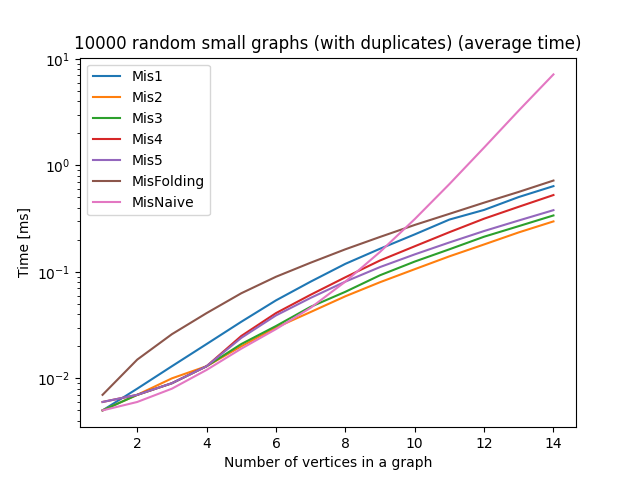
\includegraphics[width=\textwidth]{4_benchmark/plots/small.png}
\centering
\end{figure}

\begin{figure}[H]
\vspace{-1cm}
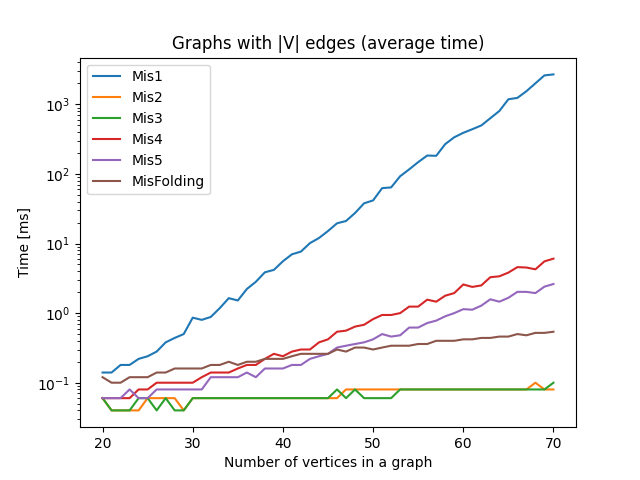
\includegraphics[width=\textwidth]{4_benchmark/plots/1n.png}
\centering
\end{figure}

\begin{figure}[H]
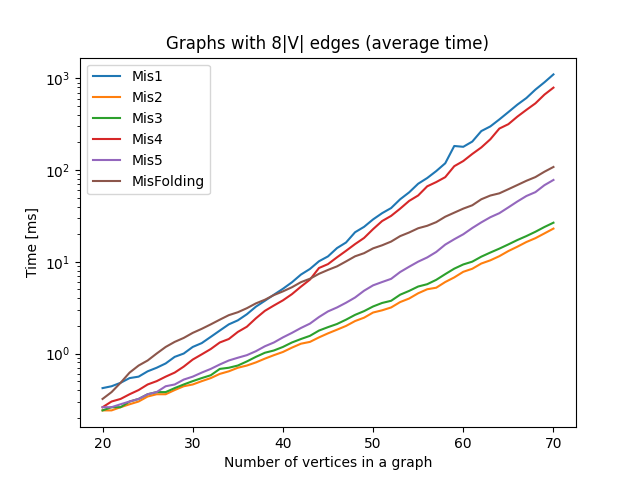
\includegraphics[width=\textwidth]{4_benchmark/plots/8n.png}
\centering
\end{figure}

\begin{figure}[H]
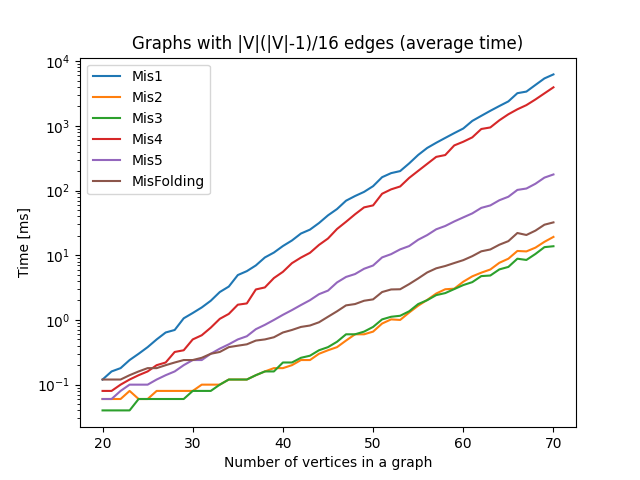
\includegraphics[width=\textwidth]{4_benchmark/plots/0.0625n2.png}
\centering
\end{figure}

\begin{figure}[H]
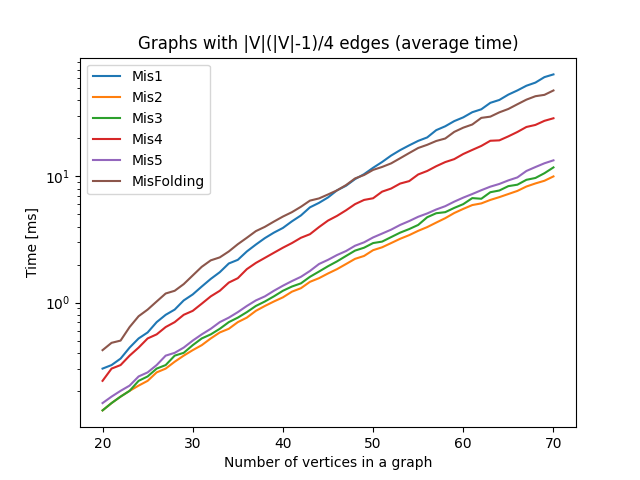
\includegraphics[width=\textwidth]{4_benchmark/plots/0.25n2.png}
\centering
\end{figure}

\begin{figure}[H]
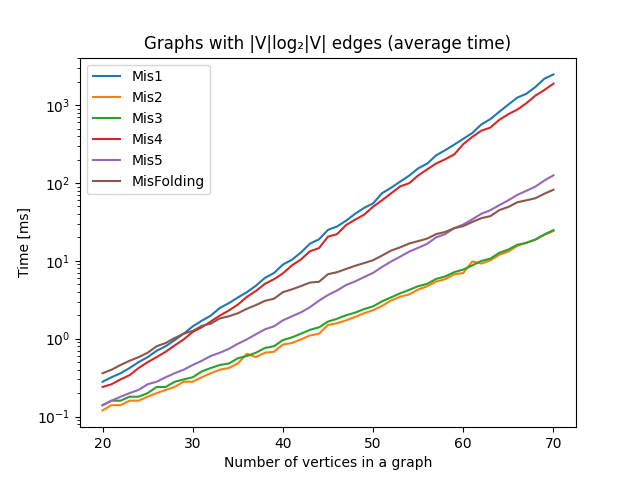
\includegraphics[width=\textwidth]{4_benchmark/plots/1nlogn.png}
\centering
\end{figure}

\begin{figure}[H]
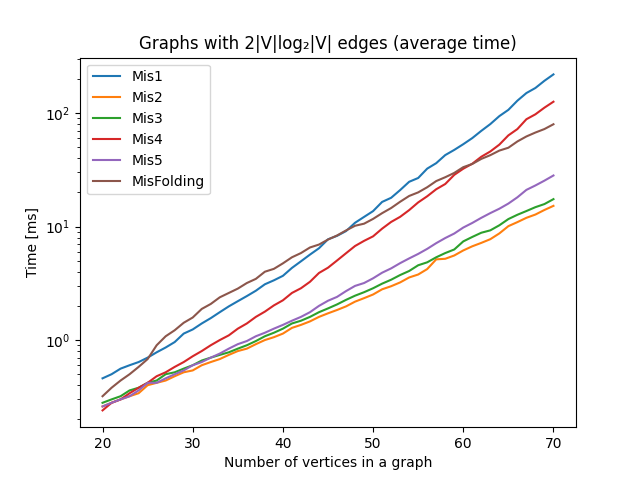
\includegraphics[width=\textwidth]{4_benchmark/plots/2nlogn.png}
\centering
\end{figure}

\begin{figure}[H]
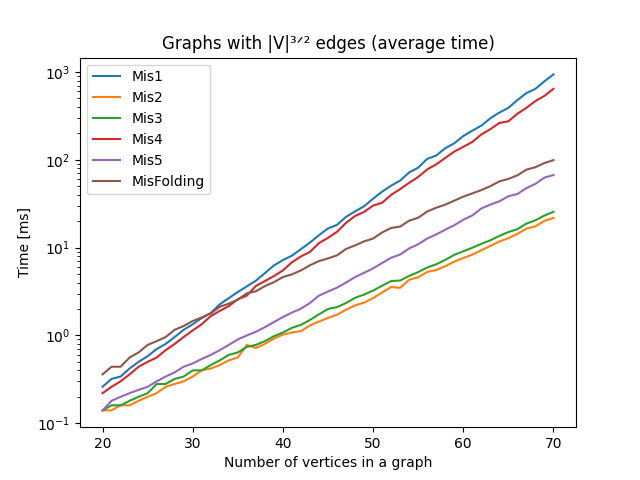
\includegraphics[width=\textwidth]{4_benchmark/plots/1n32.png}
\centering
\end{figure}

\begin{figure}[H]
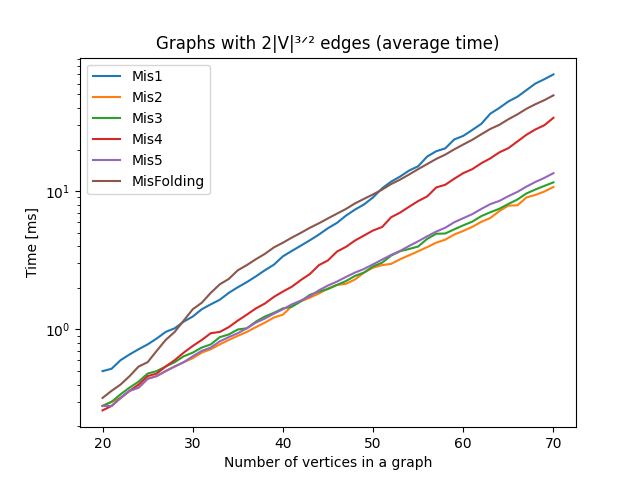
\includegraphics[width=\textwidth]{4_benchmark/plots/2n32.png}
\centering
\end{figure}

\begin{figure}[H]
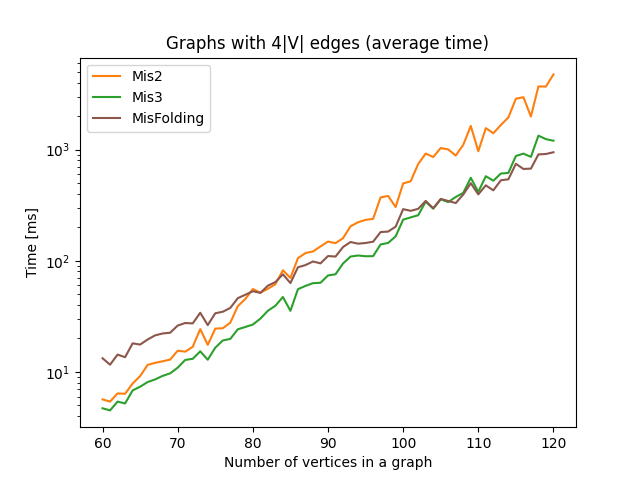
\includegraphics[width=\textwidth]{4_benchmark/plots/big4n.png}
\centering
\end{figure}

\begin{figure}[H]
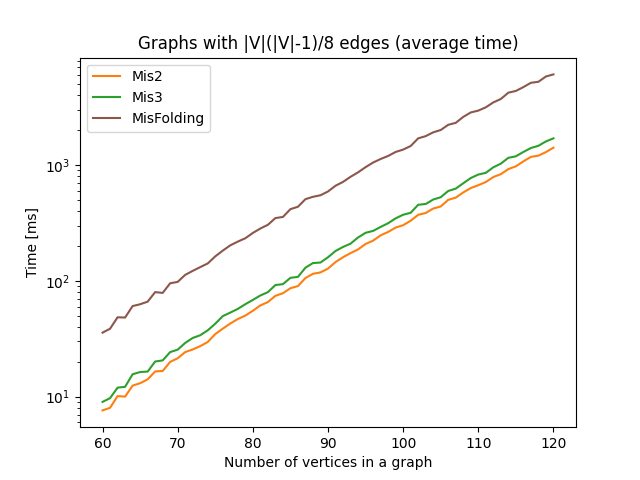
\includegraphics[width=\textwidth]{4_benchmark/plots/bign2.png}
\centering
\end{figure}

\begin{figure}[H]
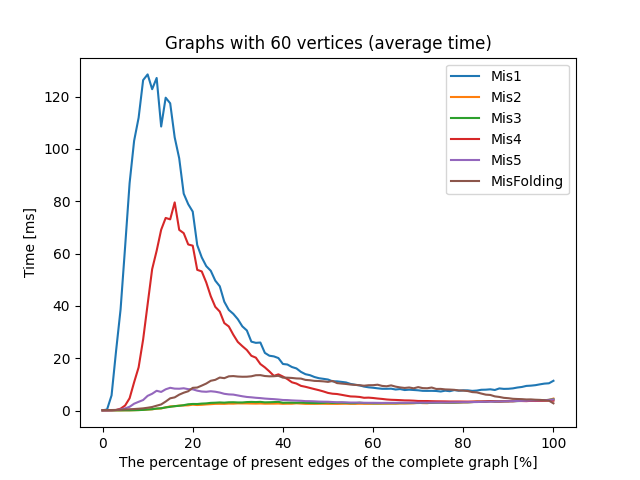
\includegraphics[width=\textwidth]{4_benchmark/plots/edges.png}
\centering
\end{figure}

\begin{figure}[H]
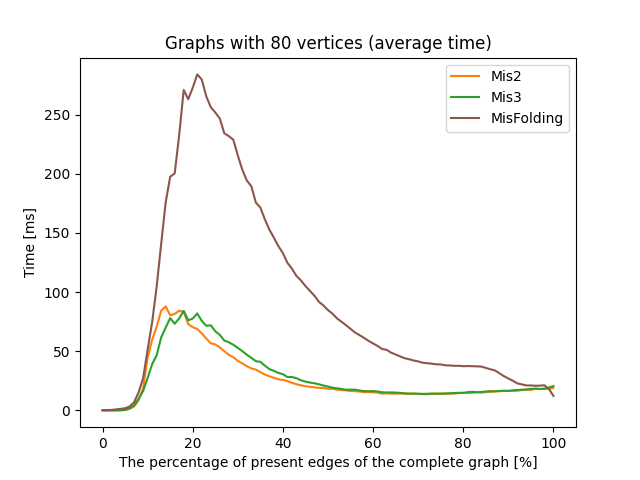
\includegraphics[width=\textwidth]{4_benchmark/plots/edges2.png}
\centering
\end{figure}


From the benchmarks performed, we can see that \textsc{MisNaive} is the slowest already for graphs as small as 10 vertices.

\textsc{Mis2} and \textsc{Mis3} are almost always the fastest for graphs up to about 100 vertices. \textsc{Mis3} algorithm is much simpler than \textsc{Mis2} but it offers a similar performance. To have a high-performance algorithm for graphs of these sizes (without much hassle) it is probably best to implement \textsc{Mis3} algorithm as well as data structures from scratch. NetworKit library has its limitations because it has to work well for all purposes. It does not perform well when graphs are heavily modified and recursion in our algorithms removes all vertices and edges.

As for graphs of higher sizes, we can see that \textsc{MisFolding} slowly gains an edge over \textsc{Mis2} and \textsc{Mis3}, at least in some specific cases. Unfortunately, we were not able to test it for graphs with larger order due to the long computing time.


\addappheadtotoc

\printbibliography

\end{document}